\section{Motivation and Observation}
\label{sec:observation}

In this section, we will first analyze the major challenges from the perspective of processing time and storage space of {\lfea}s. Then, we will give out our major observations, which are also our motivation.



\subsection{Motivation}

Due to high-accuracy and robustness, {\lfea}s have been widely used in real-world applications. As shown in Figure~\ref{fig:workflow}, they generally consist of two stages: detection and description.  An overview of their processing flow is shown as follows:


\begin{figure}[!ht]
	\centering
	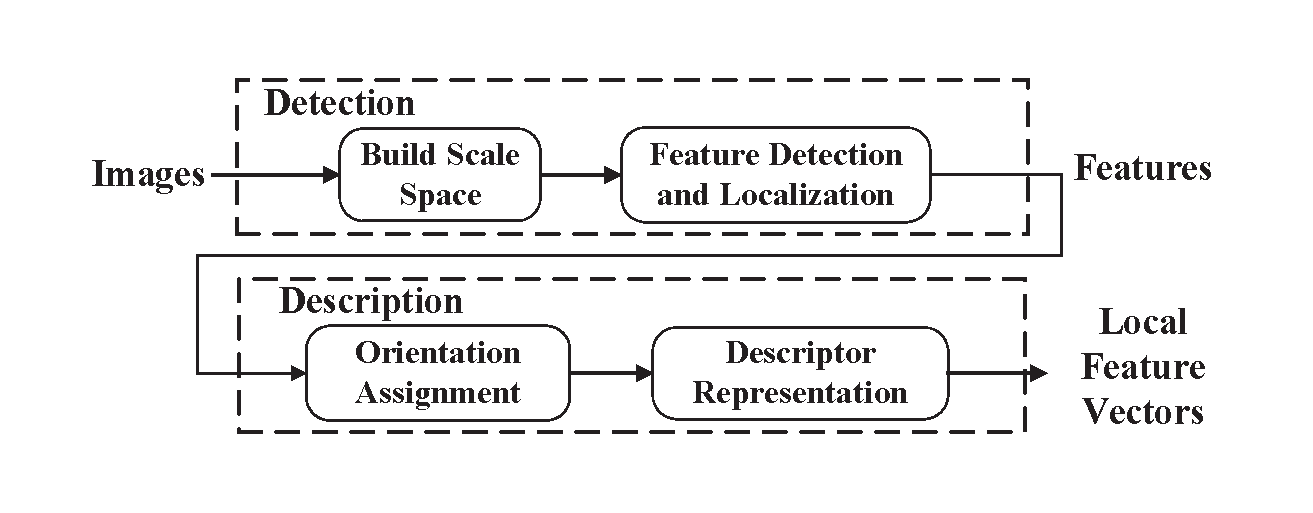
\includegraphics[width=3.8in]{images/fig-workflow.eps}
	\caption{Process flow of a typical local feature descriptor.}
	\label{fig:workflow}
\end{figure}


\begin{figure*}[!ht]
	\centering
	\subfigure[Salient region has the densest local features.]{
		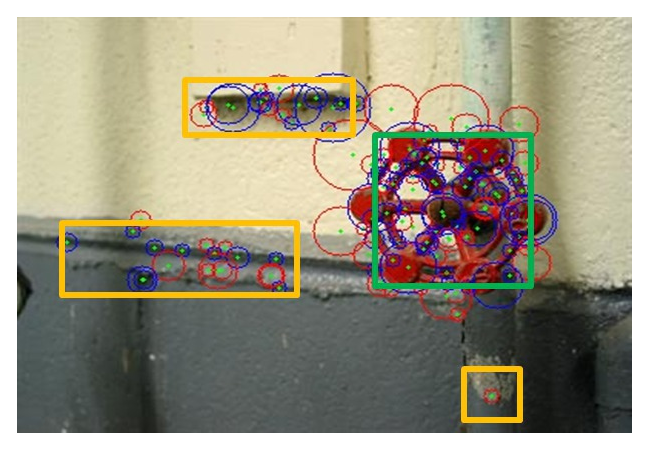
\includegraphics[width=2.2in]{images/fig-observation1.eps}
		\label{fig:observation_1}
	}
	\hfil
	\subfigure[Several salient regions in one image.]{
		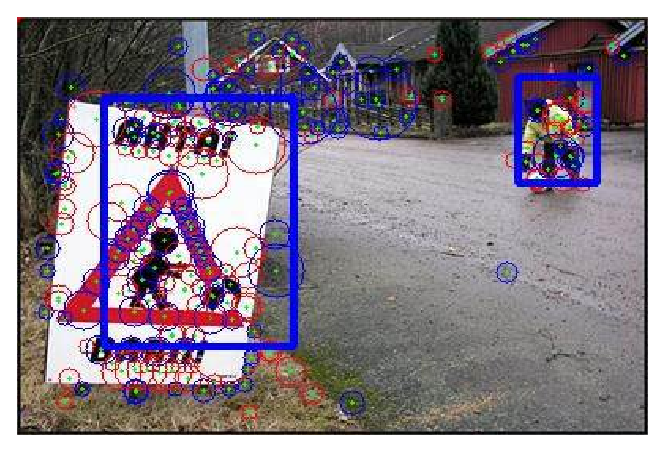
\includegraphics[width=2.2in]{images/fig-observation2.eps}
		\label{fig:observation_2}
	}
	\caption{Example images with local feature based salient regions}
	\label{fig:observations}
\end{figure*}

\squishlist

\item \textbf{Feature Detection:} This stage is to detect \emph{feature points} in an image or a video frame. After an image is initialized, a \emph{m*n} scale space pyramid is constructed to guarantee scale invariant.  After building the scale pyramid, each point in the pyramid is compared with its surrounding 26 points in a 3*3*3 cubic. If its value is the extreme value~(maximum or minimum), the point is chosen as a feature point candidate. To guarantee the quality of extracted points, the candidate points with low contrast or localized along the edges will be discarded. The remaining points are the final feature points.

\item \textbf{Feature Description:} In this stage, each detected point will be described in a high-dimensional vector. First, to make the algorithm rotation invariant, an orientation value is calculated based on the information around it. Then, a descriptor window is constructed and the vector is computed based on the orientation information. The vector value is also normalized to keep the algorithm illumination invariant.
\squishend

There exist two major issues for these {\lfea}s:
\squishlist
\setlength{\itemsep}{0mm}

\item \textbf{Performance issue:} The processing speed of these {\lfea}s are very slow and among their two stages, description stage is more time-consuming as analyzed in \cite{chen2012adaptive}.

\item  \textbf{Storage issue:} {\lfea} usually extract hundreds of feature points to represent an image and use a multi-dimensionality vector~(64 dimension for SURF\cite{bay2006surf} and 128 dimension for SIFT\cite{lowe1999object, lowe2004distinctive}) to represent a feature point, the space requirement is also high to store such a great amount of features.

\squishend

To illustrate these two problems, we evaluate the processing time, the space requirement, the point number and the proportion of execution time between two stages based on the two most widely used algorithms SIFT and SURF which are executed on a i7 Core CPU 4G memory server. The data set was used in ~\cite{mikolajczyk2005performance}. As the data shown in Table \ref{tab:surfandsift}, it can only process less than five images per second and the processing time of description stage is at least twice compared to that of the detection stage. Moreover, there are about one thousand points in each image averagely and each image requires about several hundred KB to storage its feature points.


\begin{table}[!ht]
\begin{center}
\begin{tabular}{|l|c|c|c|c|}
\hline
 & Time(ms) & Space(KB) & Pnum & Proportion \\
\hline
SURF & 171 & 269 & 989   &  1:2\\\hline
SIFT & 719 & 1437 & 2723 & 1:3 \\\hline
\end{tabular}
\end{center}
\caption{Typical time and space consumption of local feature descriptor.}
\label{tab:surfandsift}
\end{table}

As the result shown, for these {\lfea}s, the processing time and the storage space is proportional to the amount of feature points. Less feature points means less processing time and less storage space. In an image or a video frame, there exist some human visual attention regions, called salient regions, these regions are the representative parts in an image or a video frame. If only the feature points in salient regions are extracted, the image can still be represented well and the storage pressure can be released as well. There have been many salient region detection techniques~\cite{cheng2011global,achanta2009frequency,itti1998model}, which picks up visual attention parts from an image. However, prior salient region algorithms cannot satisfy the requirements in terms of processing speed and accuracy. The major constraints come from two aspects:
\squishlist
\item \textbf{Limitation of processing speed:} The goal of a typical salient region algorithm is to detect the visual attention region precisely. Therefore these prior algorithms generally include complex computation, which leads to slow processing speed.

\item \textbf{Limitation of accuracy:} In {\lfea}s, a feature point generally is a extreme point in its local region due to its high contrast. Therefore a lot of local features locate on objects' edges and corners where are also boundaries of salient regions. Since these typical salient region algorithms try to fix the region boundaries precisely, it means the feature points near the boundary cannot be guaranteed to be remained for later retrieval, which would decrease the retrieval accuracy.
\squishend


\subsection{Observation}
\label{subsec:observation}



To overcome these obstacles, we analyze the relation between the salient region and the distribution of feature points in images. We get three major observations:

\begin{description}
	
\item[Observation 1] \desclabel{itm:observation_1} \textit{There exist much denser local features in the salient regions.} It means local features we care about locates close to each other, while noisy features or unimportant features are outside and keep a distance away from them. As shown in Figure \ref{fig:observation_1}, local features in the salient region (green box) gather together and many obviously unimportant points locate far away from that box. Furthermore, our experiment based on 5000 image from~\cite{liu2011learning} show that features points in salient region can be 26 times denser than outside region at most and 3.3 times denser on average.

\item[Observation 2] \desclabel{itm:observation_2} \textit{There may exist several {\sregion}s in an image.} In other words, there exists several clusters of local features in an image. For example, the photo in Figure \ref{fig:observation_2} contains two objects, a person and a stop sign, which shape two {\sregion}s following two clusters of local features.

\item[Observation 3] \desclabel{itm:observation_3} \textit{Local features are close to boundaries of typical salient regions.} From both Figure \ref{fig:observation_1} and Figure \ref{fig:observation_2}, we can observe that most local features locate at objects' edges and corners, which are also the boundaries of typical salient regions.

\end{description}

Observation~\ref{itm:observation_1} indicates that we can detect salient regions directly based on the distribution of local features. In addition, Observation~\ref{itm:observation_2} means it's necessary to deal with the situation of multiple salient regions with multiple clusters of local features in an image. Finally, Observation~\ref{itm:observation_3} shows it's important to avoid eliminating local features on salient regions' boundaries, which require to enlarge actual salient regions to remain these boundary features.
